\section{Problem 3}
\label{part3}
\begin{verbatim}
Cluster the blogs using K-Means, using k=5,10,20. (see slide
18).  Print the values in each centroid, for each value of k.  How
many interations were required for each value of k?

\end{verbatim}
\subsection{Solution}
\begin{enumerate}

\item In this question I was asked to cluster the blogs using K-Means, using K=5,10,20. 
\item For doing this I used ``clusters.py'' code from Programming Collective Intelligence text.
\item My code for printing the values in each centroid and the number of iterations can be found in the fig\ref{lst:q3-1}.
\item Number of Iterations for K=5 is 6.
\item Number of Iterations for K=10 is 7.
\item Number of Iterations for K=20 is 6.
\item These Iterations count change if we execute the program again. Sample list of list of Iterations can be found in the fig\ref{Sample3t1}.

\newpage
\end{enumerate}
\subsection{Code Listing}

\lstinputlisting[language=Python,breaklines = true,frame=single,caption={Python Code for generating top 5 and least 5 movie recommendations that my substitute should see}, label=lst:q3-1,captionpos=b,numbers=left,showspaces=false,showstringspaces=false,basicstyle=\footnotesize]{q3.py}
\newpage

\subsection{Output}
\subsubsection{Sample output file}
\begin{figure}[ht]    
    \begin{center}
        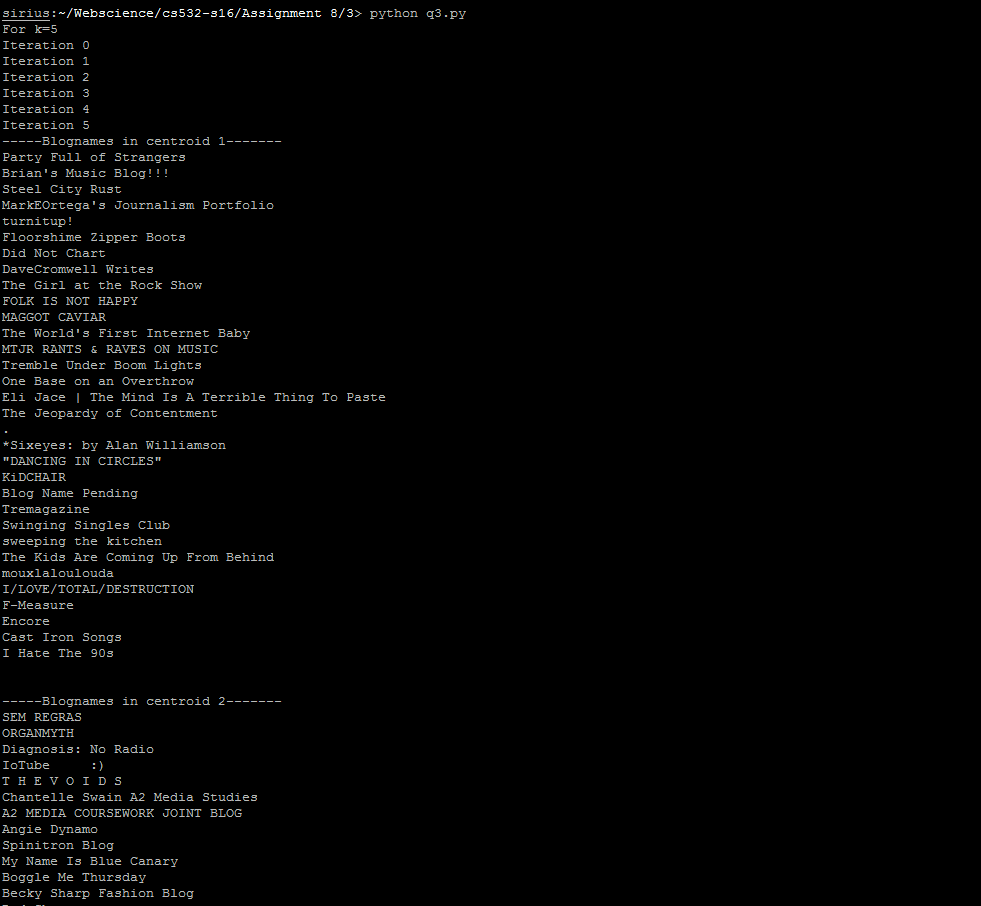
\includegraphics[scale=0.7]{output_q3.png}
        \caption{Sample values in each centroid and the number of iterations}
        \label{Sample3t1}
    \end{center}
\end{figure}
\newpage
